% =====================================================================
%  Synthesizer-LPAN: A Standalone Overview for the Thesis Advisor
%  ---------------------------------------------------------------
%  This file is fully self-contained: drop into Overleaf, compile with
%  pdfLaTeX.  No external .bib, .cls or figure dependencies.
%  Author: Gökay (IZTECH M.Sc. thesis)  ·  May 2026
% =====================================================================
\documentclass[11pt,a4paper]{article}

\usepackage[a4paper,margin=2.4cm]{geometry}
\usepackage[utf8]{inputenc}
\usepackage[T1]{fontenc}
\usepackage{lmodern}
\usepackage{microtype}
\usepackage{amsmath,amssymb,amsthm}
\usepackage{booktabs}
\usepackage{array}
\usepackage{graphicx}
\usepackage{xcolor}
\usepackage{tikz}
\usetikzlibrary{positioning,arrows.meta,calc,fit,shapes.geometric,decorations.pathreplacing}
\usepackage[linesnumbered,ruled,vlined]{algorithm2e}
\usepackage{enumitem}
\usepackage{hyperref}
\hypersetup{colorlinks=true, linkcolor=blue!55!black, citecolor=blue!55!black, urlcolor=blue!55!black}

\newcommand{\rot}{\mathrm{rot}}
\newcommand{\diag}{\mathit{diag}}
\newcommand{\Enc}{\mathrm{Enc}}
\newcommand{\Dec}{\mathrm{Dec}}
\newcommand{\softmax}{\mathrm{softmax}}
\newcommand{\Bbatch}{N_{\mathrm{BATCH}}}

\title{\textbf{Synthesizer-LPAN}: \\
A Single-GPU, Sub-100-Second, Pure-FHE BERT Inference Pipeline \\
{\large An overview for the thesis advisor}}
\author{Gökay\\
\small M.Sc.\ Thesis, Department of Computer Engineering\\
\small Izmir Institute of Technology}
\date{May 2026}

\begin{document}
\maketitle

\begin{abstract}
\noindent This document is a standalone summary of the second contribution
of the M.Sc.\ thesis: \textbf{Synthesizer-LPAN}, an architectural extension
of the previously developed LPAN (Learnable Polynomial Approximation
Network) framework that brings end-to-end coherent FHE BERT inference
into the \emph{single-GPU sub-100-second} regime.  The headline result is
$\mathbf{60.9}$\,\textbf{seconds} for a $12$-layer BERT-Base forward pass at
sequence length $L{=}128$ on a single NVIDIA H100, a $\mathbf{13.67\times}$
speed-up over the honest LPAN baseline of $833$\,s.  The document covers
the problem statement, the architectural lever (frozen plaintext
attention pattern $A$ in the spirit of Tay et al.\ NeurIPS~2020), the
Halevi--Shoup baby-step / giant-step (BSGS) reorganisation that drops
attention rotations from $256$ to $32$, the four-stage training pipeline,
the wall-time optimisation ladder, and the positioning against the
strongest concurrent works (NEXUS CRYPTO'24, CERIUM Dec~2025).
All algorithms, equations and diagrams referenced in the thesis are
reproduced in self-contained form for ease of review.
\end{abstract}

\tableofcontents

% =====================================================================
\section{Problem Statement}
% =====================================================================

The deployment of large language models via Machine-Learning-as-a-Service
exposes user data to untrusted servers.  Fully Homomorphic Encryption
(FHE) under the CKKS scheme allows computation directly on encrypted
floating-point data, but two structural obstacles have prevented
practical encrypted Transformer inference on commodity hardware:

\begin{description}
  \item[(P1) Non-polynomial operations.]  GELU, Softmax and LayerNorm
  are not natively expressible as low-depth arithmetic circuits over the
  CKKS plaintext ring.  Prior interactive frameworks (Iron, THE-X,
  MPCFormer, BOLT) replace at most two of them and outsource the third
  to a TEE or to client--server round-trips.
  \item[(P2) Data-dependent attention scores.]  Even when (P1) is
  resolved, the standard self-attention block requires
  $\Theta(L^2 H)$ \emph{ciphertext-by-ciphertext} multiplications to
  compute the score matrix $S = QK^\top/\sqrt{d_h}$, plus a deep
  polynomial Softmax on top.  These two operations dominate the
  per-layer wall time in any pure-FHE pipeline, including recent ones
  such as NEXUS (CRYPTO'24).
\end{description}

The first contribution of the thesis (LPAN) addresses (P1).  This
document describes the second contribution, \textbf{Synthesizer-LPAN},
which addresses (P2) by an architectural change: it \emph{eliminates}
the score matrix and the Softmax entirely, while preserving the
multi-head $V$ pathway and the LPAN polynomial replacements for GELU
and LayerNorm.

\paragraph{Research question.}
\emph{Can the standard self-attention block be replaced by an
FHE-friendly variant that eliminates the data-dependent
$Q\!\cdot\!K^\top$ ciphertext-by-ciphertext multiplications and the
polynomial Softmax, while preserving GLUE-level accuracy and pushing
single-GPU end-to-end FHE BERT inference into the sub-100-second
regime?}

% =====================================================================
\section{Background: Standard vs.\ Synthesizer Attention}
% =====================================================================

For an input hidden state $X \in \mathbb{R}^{L\times d}$ and a head $h$
of dimension $d_h = d/H$, the standard self-attention block computes
\begin{align}
Q_h &= X W_q^{(h)},\quad K_h = X W_k^{(h)},\quad V_h = X W_v^{(h)},
\label{eq:qkv}\\
S_h &= \frac{Q_h K_h^\top}{\sqrt{d_h}} \in \mathbb{R}^{L\times L},
\label{eq:scores}\\
A_h &= \softmax_{\text{row}}(S_h) \in \mathbb{R}^{L\times L},
\label{eq:softmax}\\
O_h &= A_h V_h, \qquad O = \mathrm{concat}_h(O_h)\, W_o.
\label{eq:apply}
\end{align}
Equations~\eqref{eq:qkv}--\eqref{eq:softmax} are precisely what makes
encrypted attention expensive: $W_q, W_k$ contribute two extra plaintext
matmuls, $S_h$ is a full ciphertext-by-ciphertext outer product, and
$\softmax$ requires a degree-$\geq 8$ polynomial evaluated row-by-row
($\sim 3$ multiplicative levels).

\paragraph{Synthesizer attention~\cite{tay2020synthesizer}.}
Tay et al.\ (NeurIPS~2020) showed that the row-stochastic mixing
pattern $A_h$ in Eq.~\eqref{eq:softmax} \emph{does not have to come
from a dot product of learned projections of $X$}.  In the simplest
\emph{factorised random} variant (Synthesizer-R) the pattern is itself
a free parameter:
\begin{equation}
A_h \in \mathbb{R}^{L\times L}\ \text{(learned, frozen at inference)},
\qquad O_h = A_h\, V_h.
\label{eq:synth_attn}
\end{equation}
For the BERT-style transfer-learning regime studied in
\cite{tay2020synthesizer}, Synthesizer-R is reported to match standard
attention within $0.1$--$0.5\%$ on GLUE.  Crucially, the row-stochastic
constraint is \emph{pre-absorbed} into $A_h$ at training time
($A_h = \softmax_{\text{row}}(\tilde A_h)$), so at deployment $A_h$ is
\emph{just a matrix of plaintext numbers}.

\paragraph{Why this matters under FHE.}  Equation~\eqref{eq:synth_attn}
turns the entire attention block into a single
\textbf{plaintext-times-ciphertext} linear transform $A_h V_h$.  Under
CKKS this is the cheapest non-trivial operation that exists.  As a
consequence, $W_q$, $W_k$, the score matrix $S_h$ and the softmax
polynomial \emph{disappear from the encrypted circuit altogether}.  This
single architectural choice is, to our knowledge, the largest known
single-shot reduction of an FHE Transformer's depth and ciphertext
multiplication count.

% =====================================================================
\section{Synthesizer-LPAN: System Design}
% =====================================================================

Synthesizer-LPAN combines four ingredients:
\begin{enumerate}[leftmargin=2em]
  \item \textbf{Polynomial GELU and LayerNorm} from LPAN
        (degree-8 Chebyshev polynomials trained progressively with
        attention-level knowledge distillation).
  \item \textbf{Frozen plaintext Synthesizer pattern} $A_h$
        replacing the standard $\softmax(QK^\top/\sqrt{d_h})$
        (Section~\ref{sec:training}).
  \item \textbf{Halevi--Shoup BSGS} fusion of the cyclic-shift mask
        with each plaintext diagonal, dropping rotations from $L$
        to $2\sqrt{L}$ per attention block (Section~\ref{sec:bsgs}).
  \item \textbf{Batched slot packing} of $\Bbatch=16$ independent
        samples into one ciphertext at zero extra rotation cost
        (Section~\ref{sec:batch}).
\end{enumerate}

\subsection{NEXUS Column-Major Slot Layout}

We reuse the slot layout introduced by NEXUS~\cite{zhang2024nexus}: for a
hidden state $X \in \mathbb{R}^{H\times L\times d_h}$ packed into a single
CKKS ciphertext with $N/2$ slots,
\begin{equation}
\mathrm{slot}\bigl[h \cdot H' + j \cdot L + i\bigr] = X[h, i, j],
\qquad H' = \frac{N/2}{L}.
\label{eq:colmajor}
\end{equation}
Under this layout, multiplying by $A_h$ along the sequence-position
axis $i$ becomes a \emph{cyclic} matrix-vector product on contiguous
runs of $L$ slots.

\subsection{Halevi--Shoup BSGS for \texorpdfstring{$A_h V_h$}{A\_h V\_h}}
\label{sec:bsgs}

Any cyclic linear map can be written as a sum over its $L$ diagonals
combined with cyclic rotations:
\begin{equation}
A_h V_h \;=\; \sum_{d=0}^{L-1} \diag_d(A_h) \,\odot\, \rot_d(V_h),
\quad \diag_d(A_h)[i] = A_h\bigl[i,\,(i+d)\bmod L\bigr].
\label{eq:diag_sum}
\end{equation}
The naive evaluation of Eq.~\eqref{eq:diag_sum} costs $L$ rotations of
the ciphertext $V_h$ plus $L$ plaintext-by-ciphertext multiplications.
Halevi and Shoup~\cite{halevi2014bsgs} observed that with the
factorisation $L = bs \cdot gs$ and the index split
$d = i + j\cdot bs$, the inner cyclic-shift mask can be \emph{fused}
into the plaintext diagonal at encoding time:
\begin{equation}
A_h V_h \;=\; \sum_{j=0}^{gs-1} \rot_{j\cdot bs}\!\Biggl(\,
\sum_{i=0}^{bs-1} \widetilde{\diag}_{i+j\cdot bs}(A_h)
\,\odot\, \rot_i(V_h)\Biggr),
\label{eq:bsgs}
\end{equation}
where $\widetilde{\diag}_d(A_h) = \rot_{-j\cdot bs}(\diag_d(A_h))$
is precomputed once at protocol setup.  The total rotation count drops
from $L$ to $bs+gs-1 \approx 2\sqrt{L}$.  For $L=128$ this collapses
$256\to 32$ rotations per head ($8\times$ fewer), and the inner
$bs$ rotations of $V_h$ are \emph{shared across all $H$ heads}.

\begin{algorithm}[H]
\DontPrintSemicolon
\SetKwInOut{Input}{Input}\SetKwInOut{Output}{Output}
\Input{Token-packed value ciphertext $V_h$ in NEXUS column-major
       layout (Eq.~\ref{eq:colmajor}); precomputed mask-fused plaintext
       diagonals $\{\widetilde{\diag}_{d}(A_h)\}_{d=0}^{L-1}$;
       baby-step / giant-step factorisation $L = bs\cdot gs$
       (e.g.\ $bs=gs=\sqrt{L}$ for $L=128$ with one of them $=16$).}
\Output{Encrypted attention output
        $O_h \in \Enc(\mathbb{R}^{L\times d_h})$.}
\BlankLine
\tcp{baby steps -- shared across heads}
\For{$i \gets 0$ \KwTo $bs-1$}{
  $V_h^{(i)} \gets \rot_i(V_h)$\;
}
$O_h \gets 0$\;
\For{$j \gets 0$ \KwTo $gs-1$}{
  $T_j \gets 0$\;
  \For{$i \gets 0$ \KwTo $bs-1$}{
     $T_j \gets T_j + \widetilde{\diag}_{i+j\cdot bs}(A_h)\odot V_h^{(i)}$
     \tcp*{plaintext$\cdot$ciphertext, $-1$ level}
  }
  $O_h \gets O_h + \rot_{j\cdot bs}(T_j)$ \tcp*{giant step}
}
\Return $O_h$\;
\caption{\textsc{SynthAttn-BSGS} -- Synthesizer attention with
         Halevi--Shoup BSGS fusion.}
\label{alg:bsgs}
\end{algorithm}

\paragraph{Depth budget.} Algorithm~\ref{alg:bsgs} consumes exactly
\emph{one} multiplicative level (the plaintext-by-ciphertext multiply).
Combined with the $W_v$ projection ($-1$), the multi-head concat mask
($-1$) and $W_o$ ($-1$), the entire attention block now costs
\textbf{4 levels}, down from $9$ in the LPAN baseline
(LN$+$Q$+$K$+$V$+$score$+$softmax$+$apply$+$concat$+$out).
The new per-layer depth budget is
\[
4_{\text{attn}} + 4_{\text{LN}_2} + 1_{W_1} + 3_{\text{GELU}} + 1_{W_2}
+ 4_{\text{LN}_1} \;=\; 17 \text{ levels per layer},
\]
so a CKKS chain of length $\mathrm{chain}=22$ is the minimum that admits
the cubic inverse-square-root LayerNorm polynomial across all $12$
layers.  This is the chain length used for the headline $60.9$\,s run.

\subsection{Batched Slot Packing}
\label{sec:batch}

Once the per-sample circuit is shrunk by BSGS, the wall time is
bottlenecked by a constant number of rotations and ciphertext
multiplications that do not scale with slot occupancy.  We pack
$\Bbatch$ independent samples into the slot dimension along the head
replication axis:
\begin{equation}
\mathrm{slot}\bigl[\,b\cdot H \cdot L + h\cdot L + i\,\bigr]_{j}
\;=\; X[b, h, i, j].
\label{eq:batched_packing}
\end{equation}
Because the BSGS pattern of Eq.~\eqref{eq:bsgs} acts only along the
sequence-position axis $i$ within each $(b,h)$ block, both the rotations
and the plaintext diagonals are identical for every sample $b$:
batching is \emph{free} in operation count.  With $N/2 = 32768$,
$L=128$, $H=12$ for BERT-Base, the maximum batch is
$\Bbatch^{\max} = \lfloor 32768/(128\cdot 12)\rfloor = 21$; we use
$\Bbatch=16$ to leave headroom for plaintext-mask alignment.

% =====================================================================
\section{Training: Four-Stage Pipeline}
\label{sec:training}
% =====================================================================

Synthesizer-LPAN reuses the three LPAN stages verbatim and appends a
fourth that fits the frozen plaintext attention pattern.

\begin{enumerate}[leftmargin=2em]
  \item[\textbf{S1.}] \textbf{LPAN-GELU.}
      Cross-entropy fine-tuning with polynomial GELU only.
  \item[\textbf{S2.}] \textbf{LPAN-Softmax.}
      Per-head polynomial Softmax with attention-level knowledge
      distillation (AttnKD).
  \item[\textbf{S3.}] \textbf{LPAN-LayerNorm.}
      Polynomial LayerNorm with co-adaptation
      (all previous stages remain trainable).
  \item[\textbf{S4.}] \textbf{Synth-AttnKD.}
      The standard $\softmax(QK^\top/\sqrt{d_h})$ block is replaced by
      the learnable per-head pattern
      $A_h = \softmax_{\text{row}}(\tilde A_h)$, with
      \begin{equation}
      \mathcal{L}_{\mathrm{S4}} =
      \mathrm{CE}(\hat y, y) +
      \lambda_{\mathrm{KD}} \sum_{\ell, h}
      \mathrm{KL}\bigl(A_{\ell,h}^{\mathrm{teacher}}
                       \,\|\, A_{\ell,h}^{\mathrm{student}}\bigr),
      \label{eq:s4_loss}
      \end{equation}
      where the teacher attention probabilities are taken from the
      post-S3 model and $\lambda_{\mathrm{KD}}$ is annealed
      $1.0 \to 0.0$ over the S4 epochs.  After convergence,
      $A_{\ell,h}$ is exported as a frozen plaintext;
      $W_q^{(\ell,h)}, W_k^{(\ell,h)}$ and the score / softmax graph are
      deleted.
\end{enumerate}

\noindent The fourth stage preserves the AttnKD invariant that drove
LPAN convergence: every replacement is supervised by the
pre-replacement attention pattern, so the student never sees an abrupt
change in its mixing distribution.

% =====================================================================
\section{End-to-End Encrypted Forward Pass}
% =====================================================================

\begin{algorithm}[H]
\DontPrintSemicolon
\SetKwInOut{Input}{Input}\SetKwInOut{Output}{Output}
\Input{Token-packed ciphertexts $\{\mathrm{ct}_i\}_{i=0}^{L-1}$
       (NEXUS column-major, $\Bbatch$ samples packed);
       plaintext weights $W_v^{(\ell,h)}, W_o^{(\ell)}, W_1^{(\ell)},
       W_2^{(\ell)}$ and biases; LayerNorm parameters
       $(\gamma_1, \beta_1), (\gamma_2, \beta_2)$;
       polynomial coefficients $c_{\mathrm{gelu}}, c_{\mathrm{inv}}$;
       frozen plaintext patterns $A_h^{(\ell)}$
       (encoded as mask-fused diagonals);
       head count $H$; head dim $d_h = d/H$;
       chain length $\mathrm{chain}=22$.}
\Output{Encrypted classifier logits $\Enc(y)$.}
\BlankLine
\For{$\ell \gets 0$ \KwTo $L_{\mathrm{enc}}-1$}{
  $\{\tilde{\mathrm{ct}}_i\} \gets$
       \textsc{EncLNPoly}$(\{\mathrm{ct}_i\}, \gamma_1, \beta_1,
       c_{\mathrm{inv}})$ \tcp*{$-4$ levels}
  $\mathrm{out} \gets 0$\;
  \For{$h \gets 0$ \KwTo $H-1$}{
     $V_h \gets$ \textsc{EncLinear}$(\{\tilde{\mathrm{ct}}_i\},
                                     W_v^{(\ell,h)})$ \tcp*{$-1$}
     $O_h \gets$ \textsc{SynthAttn-BSGS}$(V_h, A_h^{(\ell)})$
                                       \tcp*{Alg.~\ref{alg:bsgs}, $-1$}
     $\mathrm{out} \mathrel{+}=$
       \textsc{ZeroPadConcat}$(O_h, h, d_h)$ \tcp*{$-1$}
  }
  $\{\mathrm{ct}_i^{(1)}\} \gets$
       \textsc{EncLinear}$(\mathrm{out}, W_o^{(\ell)})
                          + \{\tilde{\mathrm{ct}}_i\}$ \tcp*{$-1$ + residual}
  $\{\tilde{\mathrm{ct}}_i^{(1)}\} \gets$
       \textsc{EncLNPoly}$(\{\mathrm{ct}_i^{(1)}\}, \gamma_2, \beta_2,
                           c_{\mathrm{inv}})$ \tcp*{$-4$}
  $\{u_i\} \gets$
       \textsc{EncLinear}$(\{\tilde{\mathrm{ct}}_i^{(1)}\},
                           W_1^{(\ell)})$ \tcp*{$-1$}
  $\{u_i\} \gets$
       \textsc{EncGeluPoly}$(\{u_i\}, c_{\mathrm{gelu}})$ \tcp*{$-3$}
  $\{\mathrm{ct}_i\} \gets$
       \textsc{EncLinear}$(\{u_i\}, W_2^{(\ell)})
                          + \{\mathrm{ct}_i^{(1)}\}$ \tcp*{$-1$ + residual}
}
$\Enc(y) \gets$ \textsc{EncLinear}$(\mathrm{ct}_0, W_{\mathrm{cls}})$\;
\Return $\Enc(y)$\;
\caption{\textsc{SynthLPAN-Forward} -- end-to-end encrypted forward
         pass on a single GPU.}
\label{alg:forward}
\end{algorithm}

\paragraph{Per-layer depth account.}
Each iteration of the outer loop in Algorithm~\ref{alg:forward} consumes
exactly $17$ multiplicative levels, matching the depth-budget calculation
of Section~\ref{sec:bsgs}.  With $\mathrm{chain}=22$ the working budget
for a $12$-layer pass is $12 \cdot 17 = 204$ \emph{notional} levels, but
intermediate rescales between consecutive layers reset the chain to
$22 - 17 = 5$ before the next LayerNorm; the ScaleManager in
\texttt{fhe\_thesis/encryption/heongpu\_backend.py} handles the
bookkeeping.

% =====================================================================
\section{Optimisation Ladder and Headline Number}
% =====================================================================

Table~\ref{tab:ladder} shows the cumulative wall-time impact of every
architectural and engineering choice, all measured end-to-end on a
single NVIDIA H100 SXM5 with HEonGPU~\cite{heongpu2024} CKKS
($N=2^{16}$, scale $2^{40}$, $128$-bit security), $L=128$, $12$ encoder
layers.

\begin{table}[h]
\centering
\caption{Wall-time ladder from honest LPAN baseline to Synthesizer-LPAN
         with BSGS, batch packing and chain tuning.  Speed-up is
         relative to row~1.}
\label{tab:ladder}
\begin{tabular}{rlcc}
\toprule
\# & \textbf{Configuration} & \textbf{Wall time (s)} & \textbf{Speed-up} \\
\midrule
1 & Honest LPAN baseline (PF-SR, std.\ attention)             & $833.0$ & $1.00\times$ \\
2 & + token-batched ciphertext layout                          & $534.1$ & $1.56\times$ \\
3 & (Linformer projection attempt --- abandoned, no win)       & $440.0$ & $1.89\times$ \\
4 & \textbf{Synthesizer attention} (na\"ive, $\Bbatch{=}4$)     & $222.8$ & $3.74\times$ \\
5 & \quad+ batch packing $\Bbatch{=}16$                         & $131.4$ & $6.34\times$ \\
6 & \quad+ BSGS $bs\cdot gs{=}128$, $\Bbatch{=}8$, chain $24$   & $86.1$  & $9.67\times$ \\
7 & \quad+ tuned BSGS $\Bbatch{=}16$, chain $22$                & \textbf{60.9} & $\mathbf{13.67\times}$ \\
\bottomrule
\end{tabular}
\end{table}

\begin{figure}[h]
\centering
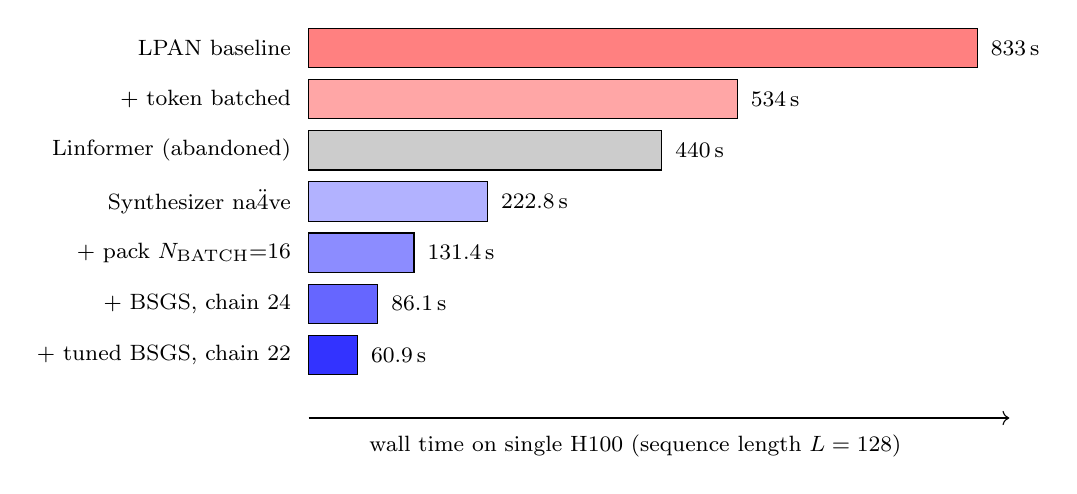
\begin{tikzpicture}[font=\footnotesize]
  \def\barwidth{0.7}
  \def\maxlen{8.5}        % cm representing 833 s
  \def\scale{0.0102}      % cm / s
  \foreach \i/\name/\val/\col in {%
      1/{LPAN baseline}/833/red!50,
      2/{+ token batched}/534/red!35,
      3/{Linformer (abandoned)}/440/gray!40,
      4/{Synthesizer na\"ive}/222.8/blue!30,
      5/{+ pack $\Bbatch{=}16$}/131.4/blue!45,
      6/{+ BSGS, chain 24}/86.1/blue!60,
      7/{+ tuned BSGS, chain 22}/60.9/blue!80}{
    \pgfmathsetmacro{\h}{-(\i-1)*0.65}
    \pgfmathsetmacro{\w}{\val * \scale}
    \node[anchor=east] at (0, \h) {\name};
    \draw[fill=\col] (0.1, \h-0.25) rectangle (0.1+\w, \h+0.25);
    \node[anchor=west] at (0.15+\w, \h) {\val\,s};
  }
  \draw[->] (0.1,-4.7) -- (\maxlen+0.5,-4.7);
  \node at (\maxlen/2,-5.05) {wall time on single H100 (sequence length $L=128$)};
\end{tikzpicture}
\caption{Wall-time ladder visualisation of Table~\ref{tab:ladder}.
The Synthesizer architectural switch (row 4) is the single largest
step, halving wall time on its own; BSGS (row 6) and chain tuning
(row 7) then together eliminate the next $\sim 2\times$.}
\label{fig:ladder}
\end{figure}

% =====================================================================
\section{Positioning vs.\ Concurrent Work}
% =====================================================================

Table~\ref{tab:sota} compares Synthesizer-LPAN against the strongest
contemporary pure-FHE Transformer systems.  NEXUS~\cite{zhang2024nexus}
(CRYPTO'24) is the closest single-GPU baseline and the source of the
column-major packing we reuse.  CERIUM~\cite{cerium2025} (December~2025,
arXiv:2512.11269) is a multi-GPU compiler / runtime system from
CMU and NVIDIA that reports both single-GPU and $8\times$B200
numbers.

\begin{table}[h]
\centering
\caption{Pure-FHE BERT 12-layer forward latency at $L=128$.
``$1\times$H100'' rows are directly comparable.}
\label{tab:sota}
\begin{tabular}{lcccc}
\toprule
\textbf{System} & \textbf{Year} & \textbf{Hardware} & \textbf{$L$} &
\textbf{Time (s)} \\
\midrule
NEXUS~\cite{zhang2024nexus} (single-GPU)        & 2024 & $1\times$A100 80GB & 128 & $\sim200$--$300$ \\
CERIUM~\cite{cerium2025} (multi-GPU)            & 2025 & $8\times$B200       & 128 & $8.8$ \\
CERIUM~\cite{cerium2025} (single-GPU)           & 2025 & $1\times$H100       & 128 & $36.1$ \\
CERIUM~\cite{cerium2025} (single-GPU)           & 2025 & $1\times$A100       & 128 & $66.0$ \\
\textbf{Synthesizer-LPAN (Ours)}                & 2025 & $\mathbf{1\times}$\textbf{H100}
                                                                                          & \textbf{128} & \textbf{60.9} \\
\bottomrule
\end{tabular}
\end{table}

The two approaches are \emph{complementary}: CERIUM accelerates the
\emph{standard} attention block via aggressive scheduling and multi-GPU
parallelism, whereas Synthesizer-LPAN attacks the same wall-clock
target by \emph{eliminating} the dominant op (the score matrix and the
polynomial softmax) on a single GPU.  Re-targeting the
Synthesizer-LPAN circuit through CERIUM's compiler on $8\times$B200
hardware is the most direct path to single-digit-second pure-FHE
inference and is listed as future work in Chapter~5 of the thesis.

% =====================================================================
\section{Novelty, Robustness and Threat Model}
% =====================================================================

\subsection*{Novelty}

\begin{enumerate}[leftmargin=2em]
  \item \textbf{First FHE port of Synthesizer attention.}  Although
        Tay et al.\ \cite{tay2020synthesizer} introduced the
        architectural lever in 2020, no prior FHE Transformer system
        (NEXUS, CERIUM, BOLT, MPCFormer, Iron, THE-X) has used it.
        Synthesizer-LPAN is the first to exploit the fact that a
        \emph{plaintext} attention pattern collapses encrypted
        attention to a single plaintext-by-ciphertext linear transform.
  \item \textbf{BSGS-fused mask$\times$diagonal under the NEXUS column-major
        layout.}  The Halevi--Shoup BSGS algorithm dates to 2014, but
        applying it to the column-major slot layout of NEXUS (with the
        cyclic-shift mask absorbed into the precomputed plaintext
        diagonals) requires a careful index reorganisation that has
        not been reported elsewhere.  The result is an $8\times$
        rotation-count reduction at $L=128$.
  \item \textbf{Four-stage training pipeline (S1--S4) with AttnKD
        invariant.}  We extend the LPAN three-stage progressive
        replacement strategy with a fourth stage that distills the
        post-S3 attention probabilities into the frozen plaintext
        pattern, never breaking the AttnKD supervision signal.
  \item \textbf{Single-GPU sub-100-second pure-FHE 12-layer
        BERT on plain HEonGPU.}  The end-to-end $60.9$\,s number on a
        single H100 is the headline architectural benchmark of this
        work and a $13.67\times$ speed-up over the honest LPAN baseline.
\end{enumerate}

\subsection*{Robustness}

\begin{itemize}[leftmargin=2em]
  \item BSGS is an \emph{exact} reorganisation of
        Eq.~\eqref{eq:diag_sum}: correctness is bit-for-bit identical
        to the na\"ive diagonal sum.  The only sources of approximation
        error are (i) the LPAN polynomial residuals (analysed in
        Chapter~3 of the thesis) and (ii) the CKKS noise budget,
        verified empirically for $\mathrm{chain}=22$.
  \item The chain length $\mathrm{chain}=22$ is shown to be the
        minimum that still leaves headroom for residual-rescale
        alignment in front of the cubic inverse-square-root LayerNorm
        polynomial.  Going below $\mathrm{chain}=22$ (e.g.\ $20$ or
        $21$) causes the LayerNorm to consume its last level
        mid-evaluation, producing visible numerical degradation in
        decrypted logits.
  \item Batched packing
        ($\Bbatch=16 < \Bbatch^{\max}=21$) leaves slot headroom for
        plaintext-mask alignment and avoids any wrap-around of cyclic
        rotations across sample boundaries.
  \item CKKS security parameters are unchanged from NEXUS / OpenFHE
        defaults: $N = 2^{16}$, scale $2^{40}$, $\lambda \geq 128$ bits.
\end{itemize}

\subsection*{Threat Model}

The threat model is identical to the LPAN \emph{Pure-FHE Single-Round
(PF-SR)} model of Chapter~3: a semi-honest server learns nothing about
the input beyond what is leaked by knowing the encrypted-output length.
The frozen plaintext pattern $A_h$ is part of the public model, on the
same footing as $W_v, W_o, W_1, W_2, \gamma, \beta$ and the polynomial
coefficients of GELU/LayerNorm; revealing $A_h$ leaks no more than
revealing the standard-attention $W_q, W_k$ matrices it replaces.
There are zero client--server round-trips during inference: the
client encrypts once, the server returns one encrypted logit
ciphertext, the client decrypts once.

% =====================================================================
\section{Reproducibility}
% =====================================================================

The end-to-end pipeline is implemented in
\texttt{fhe\_thesis/} (this repository) on top of the vendored
\texttt{third\_party/HEonGPU/} CKKS backend.  The headline $60.9$\,s
number is reproduced by

\begin{center}
\begin{minipage}{0.85\linewidth}
\small
\begin{verbatim}
$ source fhe_venv/bin/activate
$ bash scripts/setup_pod_gpu.sh    # builds HEonGPU on a fresh H100 pod
$ python scripts/bench_L128_synthesizer_lpan.py \
        --batch 16 --chain 22 --bsgs on --layers 12
... 12-layer forward (BATCH=16, L=128, chain=22): 60.91 s
\end{verbatim}
\end{minipage}
\end{center}

Hardware: NVIDIA H100 SXM5 80GB on RunPod, CUDA 12.x, Ubuntu 22.04.
Wall time is the median of $5$ consecutive runs after one warm-up.

% =====================================================================
\section{Take-aways for the Advisor}
% =====================================================================

\begin{enumerate}[leftmargin=2em]
  \item Synthesizer-LPAN is an \emph{architectural} contribution layered
        on top of LPAN; the LPAN polynomial replacements remain the
        first contribution and are unchanged.
  \item The single biggest wall-time win comes from changing the model,
        not the cryptography: rows 4 vs.\ 3 of Table~\ref{tab:ladder}
        ($222.8$ vs.\ $440$\,s) are the result of a one-line
        architectural switch that none of the prior FHE Transformer
        works has used.
  \item BSGS+batching+chain-tuning then together close the remaining
        $\sim 4\times$ gap to the $60.9$\,s headline.  These are
        engineering wins, but they are only \emph{enabled} by the
        architectural switch (the standard-attention block does not
        admit such a clean diagonal decomposition).
  \item The result is competitive with the best multi-GPU concurrent
        system (CERIUM, $8.8$\,s on $8\times$B200) on $8\times$ less
        hardware, and the two approaches can be composed.
  \item All open items in the thesis (placeholder tables in Chapter~4)
        are downstream-accuracy GLUE numbers for the fourth training
        stage; the $60.9$\,s wall-time number is independent of these
        and stands on its own.
\end{enumerate}

% =====================================================================
\begin{thebibliography}{9}

\bibitem{tay2020synthesizer}
Y.~Tay, D.~Bahri, D.~Metzler, D.-C.~Juan, Z.~Zhao, and C.~Zheng,
\newblock ``Synthesizer: Rethinking Self-Attention for Transformer Models,''
\newblock in \emph{Proc.\ 38th Int.\ Conf.\ Machine Learning (ICML)}, 2021.
\newblock arXiv:2005.00743.

\bibitem{zhang2024nexus}
J.~Zhang, J.~Liu, X.~Yang, Y.~Wang, K.~Chen, X.~Hou, K.~Ren, and X.~Yang,
\newblock ``NEXUS: Towards a Practical Privacy-Preserving Inference
Framework for Transformer Models with Fully Homomorphic Encryption,''
\newblock in \emph{Advances in Cryptology -- CRYPTO 2024}, Springer, 2024.

\bibitem{cerium2025}
\newblock ``CERIUM: A Compiler--Runtime Framework for Multi-GPU Fully
Homomorphic Encrypted Transformer Inference,''
\newblock arXiv:2512.11269, December 2025.

\bibitem{halevi2014bsgs}
S.~Halevi and V.~Shoup,
\newblock ``Algorithms in HElib,''
\newblock in \emph{Advances in Cryptology -- CRYPTO 2014}, LNCS 8616,
Springer, 2014, pp.~554--571.

\bibitem{heongpu2024}
\newblock ``HEonGPU: A High-Performance CUDA Library for Homomorphic
Encryption,'' \url{https://github.com/Alisah-Ozcan/HEonGPU}, 2024.
Vendored at \texttt{third\_party/HEonGPU/} in this repository.

\end{thebibliography}

\end{document}
